\chapter{Related Work}

This chapter highlights the foundational theories and recent advancements in the fields of remote sensing and computer vision, particularly in 
small object detection. By examining previous research that addresses similar challenges, this section not only underscores the technological 
progress achieved but also identifies the gaps that the current model aims to bridge. In the field of computer vision, Convolutional Neural Networks 
(CNNs) served as the initial models for image analysis, primarily focused on image classification where the entire image is labeled as a single 
object category. While CNNs had great performance in these tasks, their application to object detection in complex images revealed significant limitations. 



\section{Region-based Convolution Neural Networks}



\subsection{Region-based Convolution Neural Networks}

The need for more sophisticated solutions that could accurately identify and locate multiple objects within images led to the development of 
Region-based Convolutional Networks[3] (R-CNNs). Starting with the base Region-based Convolution Neural Network This approach combines region proposal 
algorithms with the feature extraction capabilities of CNNs. R-CNNs begin by generating potential object-bound regions in an image, a process known 
as region proposal. Each region is then cropped and resized to a fixed size before being fed into a pre-trained convolutional neural network. 

\begin{figure}[h!]
    \centering
    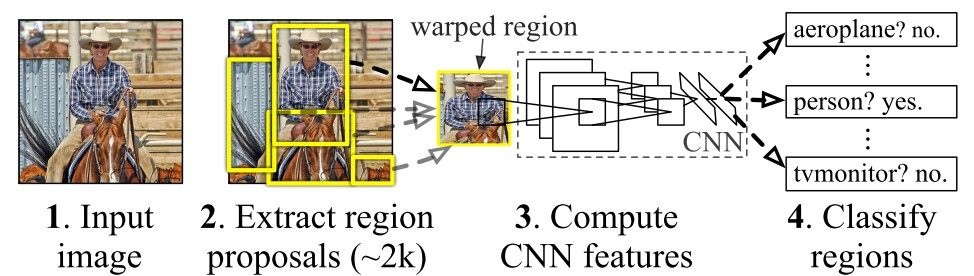
\includegraphics[scale=0.45]{Figures/rcnn.jpeg}
    \caption{Region-based Convolution Neural Network Architecture}
    \label{fig:rcnn}
\end{figure}

As we can see in the \ref{fig:rcnn} the R-CNN consists of 3 main modules. The first module generates 2,000 region proposals using the Selective Search 
algorithm. After being resized to a fixed pre-defined size, the second module extracts a feature vector of length 4,096 from each region proposal.
The third module uses a pre-trained SVM algorithm to classify the region proposal to either the background or one of the object classes.


Some the limitations of the R-CNN model are the facts that it is a multi-stage model, where each stage is an independent component, thus, it cannot be 
trained end-to-end. Also the R-CNN depends on the Selective Search algorithm for generating region proposals, which takes a lot of time and cannot be 
customized to the detection problem. Lastly each region proposal is fed independently to the CNN for feature extraction, which makes it impossible to 
run R-CNN in real-time.

\subsection{Fast Region-based Convolution Neural Networks}

Fast R-CNN improved upon the original R-CNN's efficiency, where instead of cropping and resizing each region separately, the entire image is passed through the 
CNN to extract features. Regions of interest (ROIs) are then selected from the feature map using the proposed bounding boxes from the selective search. 
These ROIs are then pooled into a fixed-size feature map and passed through fully connected layers for classification and bounding box regression as we can see 
in the figure \ref{fig:fast-rcnn}.

\begin{figure}[h!]
    \centering
    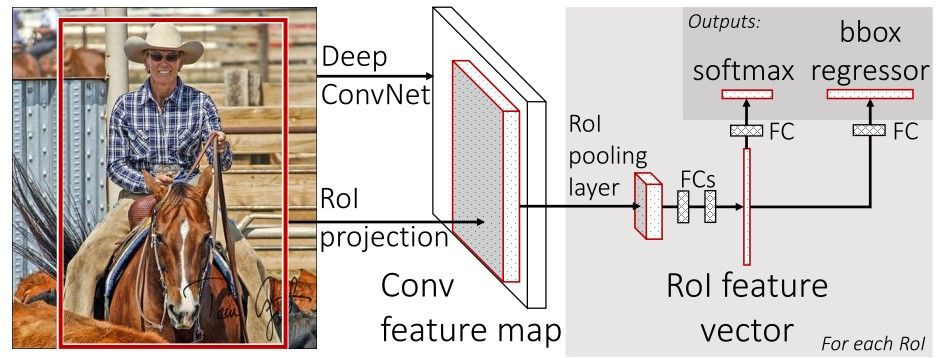
\includegraphics[scale=0.4]{Figures/fast-r-cnn.png}
    \caption{Fast Region-based Convolution Neural Network Architecture}
    \label{fig:fast-rcnn}
\end{figure}

In this model a proposed a new layer called ROI Pooling that extracts equal-length feature vectors from all proposals in the same image, where 
compared to R-CNN, which has multiple stages, Faster R-CNN builds a network that has only a single stage. 

The RoI pooling layer uses max pooling to convert the features inside any valid region of interest into a small feature map with a fixed spatial 
extent of \(H × W\) , where $H$ and $W$ are layer hyper-parameters that are independent of any particular RoI. In this paper, an RoI is a rectangular window 
into a convolution feature map. Each RoI is defined by a four-tuple \((r, c, h, w)\) that specifies its top-left corner \((r, c)\) and its height 
and width \((h, w)\). Also one of the great inclusions of this model was the implementation of multi-task loss:

\[L(p, u, t', v) = L_{cls}(p, u) + \lambda [u \geq 1] L_{loc}(t', v)z\]

,where the classification loss \(L_{cls}(p, u)\) is defined as the negative log likelihood of the true class \(u\), expressed as:
\[
L_{cls}(p, u) = -\log p_u
\]

The localization loss \(L_{loc}\) is defined over the predicted bounding box parameters \(t' = (t'_x, t'_y, t'_w, t'_h)\) and the ground truth bounding 
box parameters \(v = (v_x, v_y, v_w, v_h)\) for class \(u\). The Iverson bracket \([u \geq 1]\) is used as an indicator function that evaluates to 1 
when \(u\) is 1 or more, and 0 otherwise. This function helps in applying the localization loss only when there is a foreground class detected, 
effectively ignoring the background.

The overall loss \(L(p, u, t', v)\) is then a combination of classification and localization losses, modulated by a parameter \(\lambda\), representing the trade-off between these two tasks:
\[
L(p, u, t', v) = L_{cls}(p, u) + \lambda [u \geq 1] L_{loc}(t', v)
\]


\subsection{Faster Region-based Convolution Neural Networks}

While Fast R-CNN improved upon its predecessors in terms of both speed and accuracy, the Faster R-CNN architecture emerged as an even more refined version. 
Fast R-CNN effectively addressed the inefficiencies of previous models by integrating a region of interest (RoI)[4] pooling layer to connect convolutional 
feature extraction and region proposal tasks. However, it still relied on external region proposal algorithms, which remained a bottleneck in terms of 
computational efficiency and speed. 

\begin{figure}[h!]
    \centering
    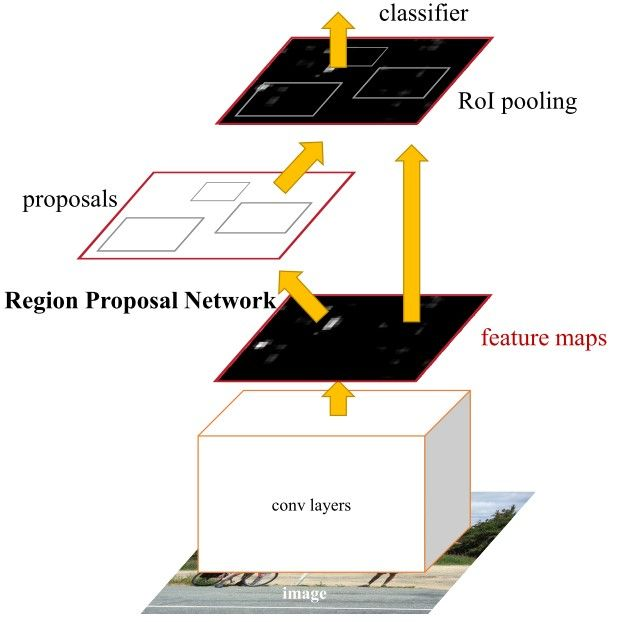
\includegraphics[scale=0.4]{Figures/faster-rcnn.jpeg}
    \caption{Faster Region-based Convolution Neural Network Architecture}
    \label{fig:faster-rcnn}
\end{figure}

Faster R-CNN resolved this by introducing a novel component, the Region Proposal Network (RPN)[5], which is a fully convolutional network that generates proposals 
with various scales and aspect ratios. The RPN implements the terminology of neural network with attention to tell the object detection where to look, 
where rather than using pyramids of images or pyramids of filters, this paper introduced the concept of Anchor Boxes. 

\begin{figure}
    \centering
    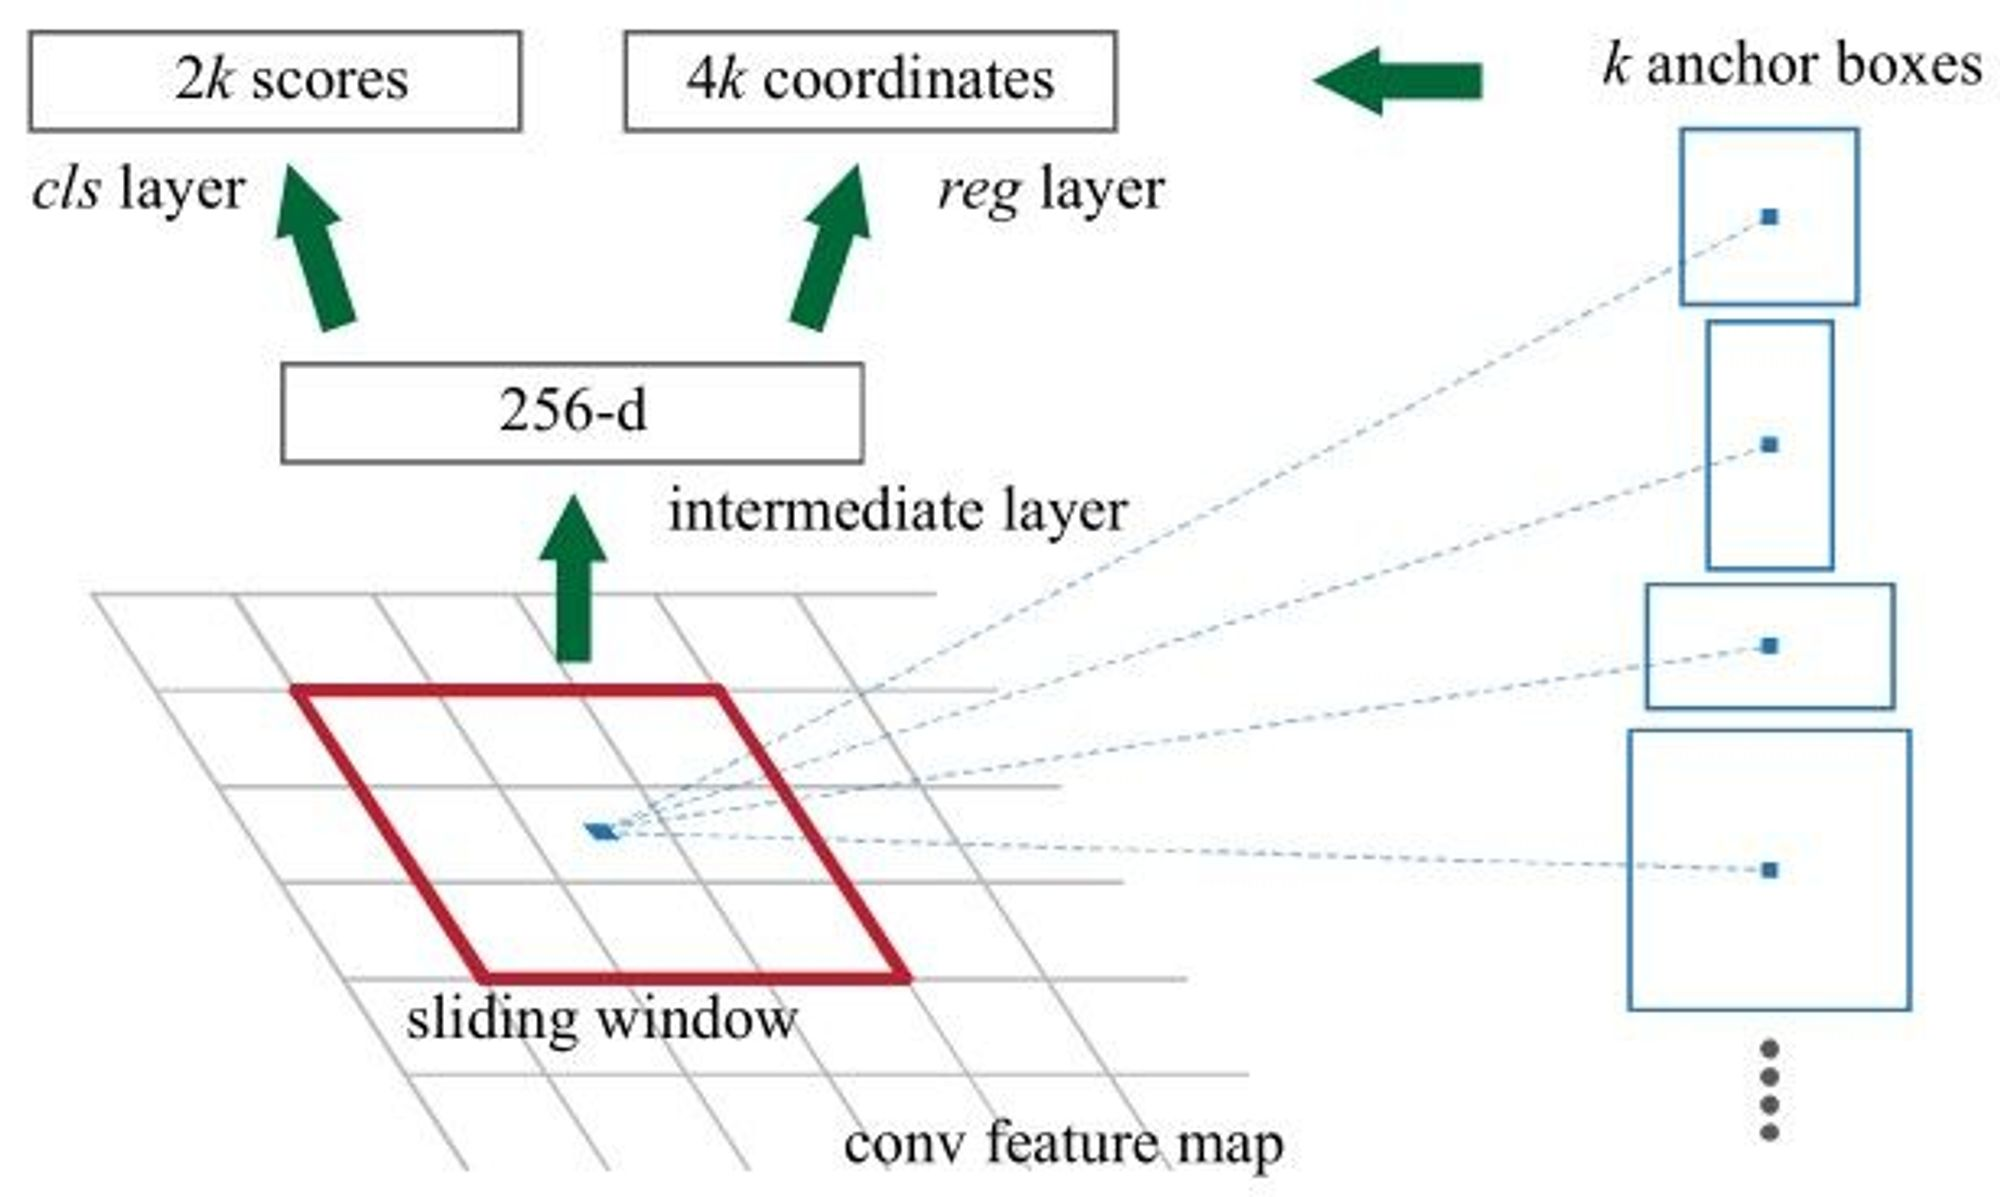
\includegraphics[scale=0.1]{Figures/anchors.jpeg}
    \caption{Anchor Boxes Generator}
    \label{fig:anchors}
\end{figure}

\newpage
An anchor box is a reference box of a specific scale and aspect ratio. With multiple reference anchor boxes, then multiple scales and aspect ratios exist 
for the single region. This can be thought of as a pyramid of reference anchor boxes. 



\subsection{Masked Region-based Convolution Neural Networks}


\section{Feature Pyramid Networks}


\subsection{Feature Pyramid Network}


\subsection{Extended Feature Pyramid Network}



\section{Vision Transformers}

\subsection{Vision Transformers}


\subsection{Masked-Attention Mask Vision Transformer}
